\section{Auswertung}

\subsection{Überprüfung der Bragg-Bedingung}

Bei der Überprüfung der Bragg-Bedingung werden in dem verwendeten Messprogramm
folgende Einstellungen für den Kristallwinkel $\vartheta$, das Zählrohrwinkelintervall
$\alpha\ua{GM}$, den Winkelzuwachs $\increment\alpha$ sowie die Integrationszeit
$\increment t$ gewählt:

\begin{align*}
  \vartheta        &= 14° \\
  \increment\alpha &= 0.1° \\
  \increment t     &= \SI{10}{s} \\
  \alpha\ua{GM}    &\in [26°, 30°] .
\end{align*}

Mithilfe von Python und der Daten aus Abbildung \ref{MessungA} wird dann das Maximum der
Impulsrate bestimmt. Der Winkel wird dann zuerst in die minimale Wellenlänge (Formel
\eqref{}) sowie
anschließend in die maximale Energie (Formel \eqref{}) umgerechnet, so dass sich folgende Werte
ergeben:

\begin{align*}
  \vartheta\ua{3.1,max} &= 28.6 ° \\
  \lambda\ua{3.1,min} &= \SI{1.93e-10}{m} \\
  E\ua{3.1, max} &= \SI{6.43}{eV} .
\end{align*}

\begin{figure}
  \centering
  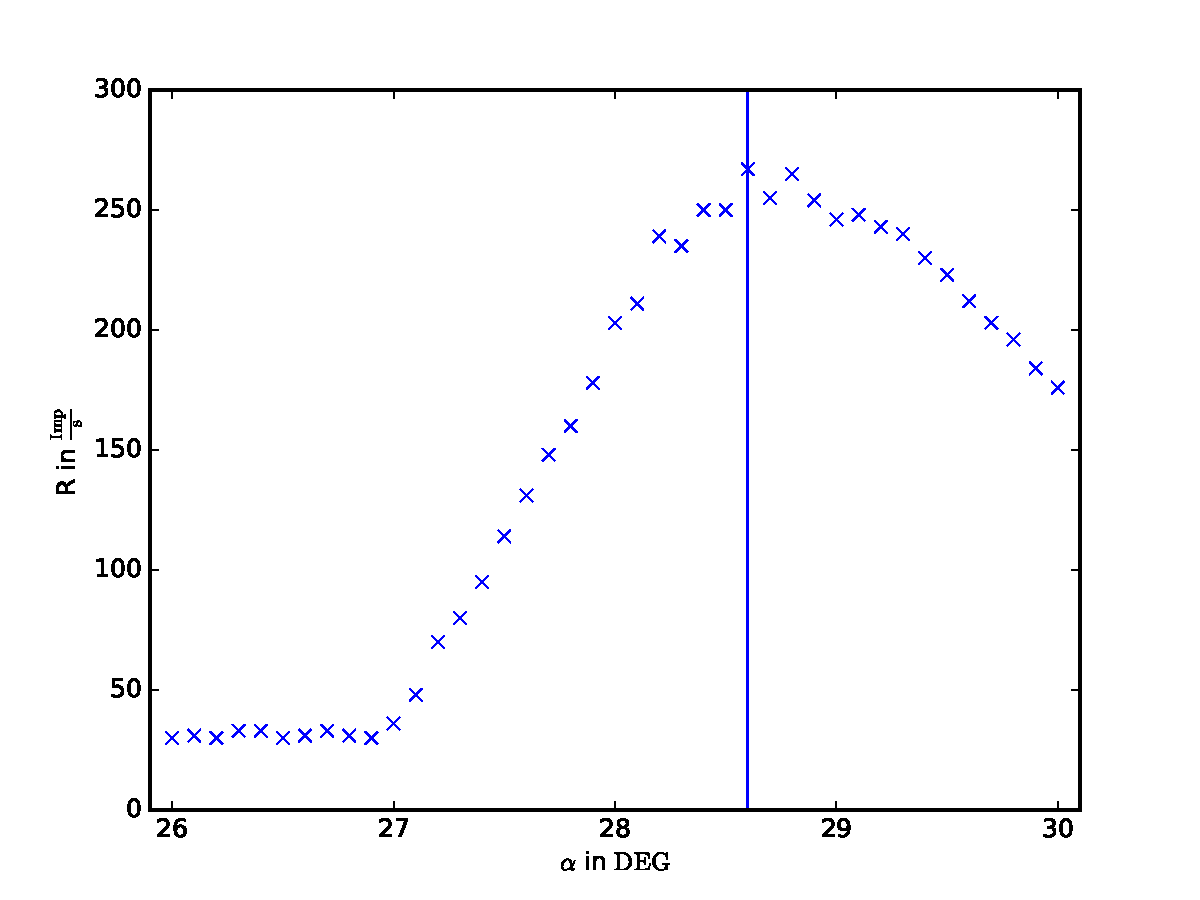
\includegraphics[width = 0.8\textwidth]{Python/MessungA.pdf}
  \caption{Gemessene Impulsrate bei Messung 3.1 .}
  \label{fig:MessungA}
\end{figure}

Im Vergleich mit dem Erwartungswert von $\vartheta$ = 14 ° ergibt sich eine
Abweichung von $\increment\vartheta$ = 0.6 ° sowie prozentual eine Abweichung
von $\increment\vartheta$ = 2.1 $\%$.

\subsection{Das Emissionsspektrum einer Cu-Röntgenröhre}

Für die Untersuchung des Emissionsspektrums einer Cu-Röntgenröhre wurden in dem
2:1 Koppelmodus die folgenden Einstellungen gewählt:

\begin{align*}
  \vartheta        &\in [4°, 26°]  \\
  \increment\vartheta &= 0.2° \\
  \increment t     &= \SI{5}{s} .
\end{align*}

Die erhaltenen Daten sind in Abbildung \ref{fig:MessungB} dargestellt. Zur Bestimmung der
$K\ua{\alpha}$- und $K\ua{\beta}$-Linie wird zuerst der Untergrund aus den Daten
herausgerechnet. Dafür wird an die Werte in Tabelle \ref{} ein Polynom 3.Ordnung
gefittet, für das sich die folgenden Parameter ergeben:

\begin{align*}
  U(x) &= A\cdot x^3 + B\cdot x^2 + C\cdot x + D \\
  A &=  (0.27 \pm 0.02) \si{\frac{Imp}{s\cdot \alpha^3}} \\
  B &= (-12.2 \pm -0.7) \si{\frac{Imp}{s\cdot \alpha^2}} \\
  C &= (170 \pm 9) \si{\frac{Imp}{s\cdot \alpha}} \\
  D &= (-525 \pm 31) \si{\frac{Imp}{s}} .
\end{align*}

Des weiteren wird an die Daten aus Tabelle \ref{} und \ref{} jeweils eine Gauß-Funktion
der Form \eqref{eqn:GaußFit} gefittet:

\begin{equation}
  G(x) = A \cdot \exp{ \frac{-(\vartheta-\vartheta_0)^2}{2\cdot s^2}} .
  \label{eqn:GaußFit}
\end{equation}

$\vartheta_0$ und $s$ geben dabei die Lage der jeweiligen Linie sowie die
Halbwertsbreite an. Damit ergeben sich für die $K\ua{\alpha}$-Linie die folgenden
Parameter:

\begin{align*}
  A\ua{K\ua{\alpha}} &= (4.7 \pm 0.3) \cdot 10^3 \si{\frac{Imp}{s}} \\
  \vartheta\ua{K\ua{\alpha}} &= \vartheta_0 =  (22.57 \pm 0.01) ° \\
  \lambda\ua{K\ua{\alpha}} &= (1.5458 \pm 0.0008) \cdot 10^{-10} \si{m} \\
  E\ua{K\ua{\alpha}} &= (8020 \pm 4) \si{eV} \\
  s\ua{K\ua{\alpha}} &= (0.19 \pm 0.1) ° .
\end{align*}

Analog ergeben sich für die $K\ua{\beta}$-Linie die folgenden Werte :

\begin{align*}
  A\ua{K\ua{\beta}} &= (1.62 \pm 0.04) \cdot 10^3 \si{\frac{Imp}{s}} \\
  \vartheta\ua{K\ua{\beta}} &= \vartheta_0 =  (20.289 \pm 0.003) ° \\
  \lambda\ua{K\ua{\beta}} &= (1.3967 \pm 0.0002) \cdot 10^{-10} \si{m} \\
  E\ua{K\ua{\beta}} &= (8876 \pm 1) \si{eV} \\
  s\ua{K\ua{\beta}} &= (0.136 \pm 0.005) ° .
\end{align*}

Mithilfe der Formeln \ref{} und \ref{} können dann die Abschirmkonstanten der K-Kante
und der L-Kante bestimmt werden, für die sich die folgenden Werte ergeben:

\begin{align*}
\sigma\ua{K} &= (3.452 \pm 0.002) \\
\sigma\ua{L} &= (17.77 \pm 0.03)
\end{align*}

Die beiden Halbwertsbreiten können nun ebenfalls in Energien umgerechnet werden.
Theoretisch sollten die beiden Energien dann exakt gleich sein. Da dies in der
Praxis jedoch nicht der Fall ist, kann mithilfe des Quotienten der beiden Energien
eine Güte des Versuches angegeben werden, dessen Optimalwert bei 1 liegt. Für
den Versuch ergibt sich damit das folgende Auflösungsvermögen:

\begin{align*}
  E\ua{s\ua{K\ua{\alpha}}} &= (9.2 \pm 0.7) \cdot 10^2 \si{eV} \\
  E\ua{s\ua{K\ua{\beta}}} &= (1.3 \pm 0.04) \cdot 10^3 \si{eV} \\
  \phi &= \frac{E\ua{s\ua{K\ua{\beta}}}}{E\ua{s\ua{K\ua{\alpha}}}} = 1.41 \pm 0.11 .
\end{align*}

\begin{figure}
  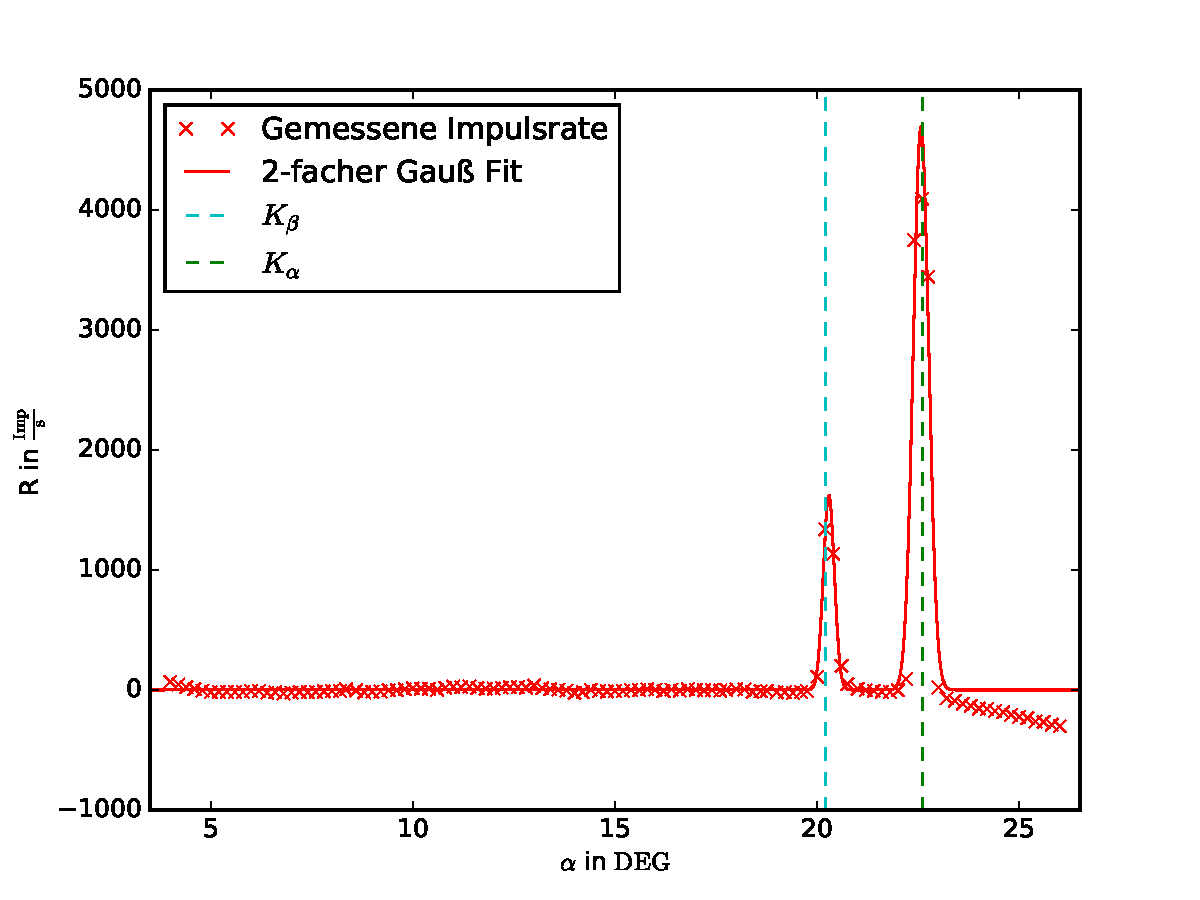
\includegraphics[width = 0.8\textwidth]{Python/MessungB.pdf}
  \caption{Gemessene Impulsrate einer Cu-Röntgenröhre}
  \label{fig:MessungB}
\end{figure}

\subsection{Das Absorptionsspektrum}

Für die Untersuchung des Absorptionsspektrums verschiedener Materialien wurden in dem
2:1 Koppelmodus die folgenden Einstellungen gewählt:

\begin{align*}
  \increment\vartheta &= 0.1° \\
  \increment t     &= \SI{20}{s} .
\end{align*}

Das Messintervall wurde dabei bei jedem Material unabhängig gewählt.

\subsubsection{Germanium}

Bei Germanium wurde ein Messintervall von $\vartheta$ $\in$ [14°, 18°] gewählt.
Mithilfe der Daten aus Tabelle \ref{} (grafisch siehe Abbildung \ref{fig:Germanium})
kann für Germanium nun die Absorptionsenergie der K-Kante bestimmt werden sowie
die daraus resultierende Abschirmkonstante nach Formel \eqref{}. Die für die Berechnung
der Werte verwendete Ordnungszahl ist 32.

\begin{figure}
  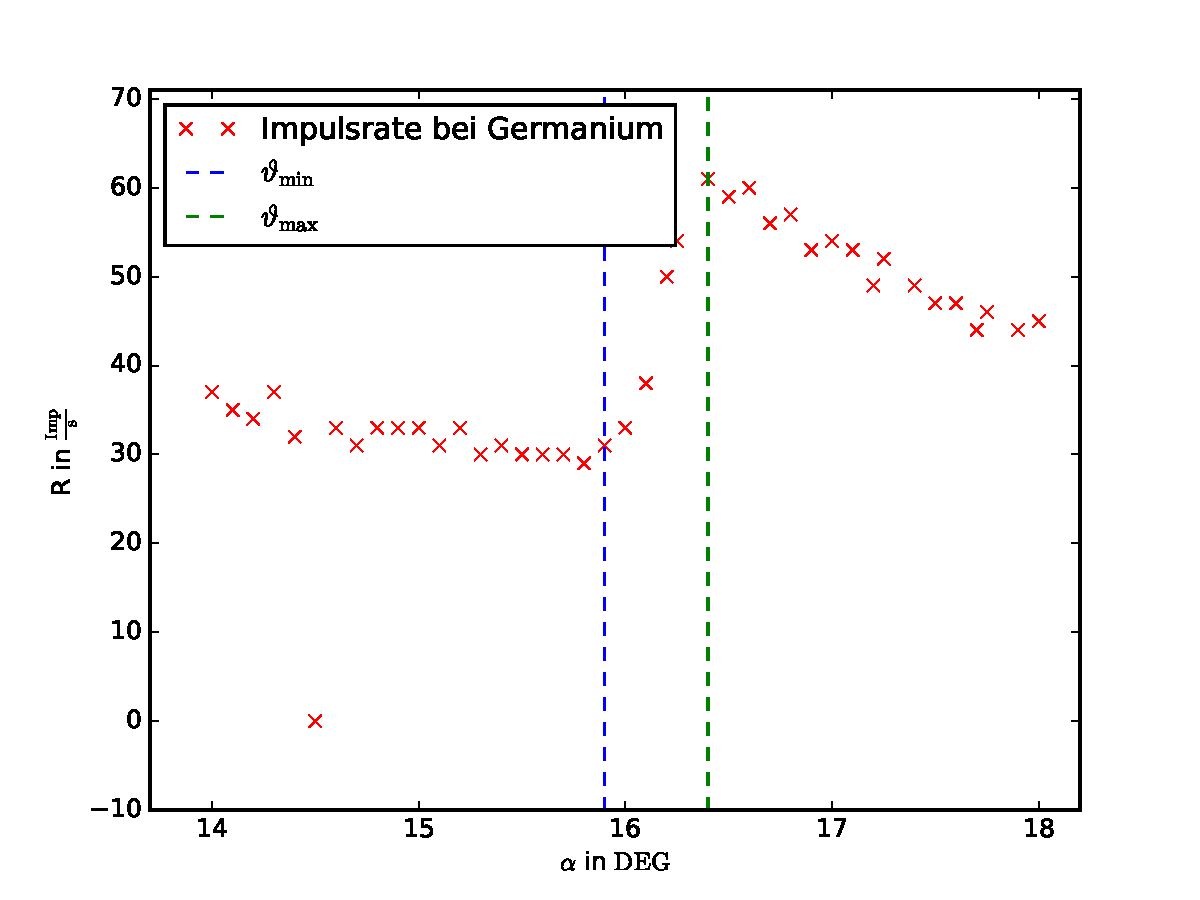
\includegraphics[width = 0.8\textwidth]{Python/Germanium.pdf}
  \caption{Gemessenes Absorptionsspektrum bei Germanium.}
  \label{fig:Germanium}
\end{figure}

\begin{align*}
  \vartheta\ua{GE} &= 16.15 ° \\
  \lambda\ua{GE,min} &= 1.12 \cdot 10^{-10} \si{m} \\
  E\ua{GE,max} &= 11066 \si{eV} \\
  \sigma\ua{GE} &= 3.72
\end{align*}

\begin{table}
  \centering
  \caption{Gemessene Impulsrate N bei Germanium.}
  \label{tab:Germanium}
  \begin{tabular}{c c | c c | c c}
    \toprule
    $\vartheta$ in deg & N in $\frac{\su{Imp}}{\su{s}}$ & $\vartheta$ in deg &
    N in $\frac{\su{Imp}}{\su{s}}$ & $\vartheta$ in deg & N in $\frac{\su{Imp}}{\su{s}}$ \\
    \midrule
    28.0 & 37.0 & 30.8 & 31.0 & 33.6 & 57.0 \\
    28.2 & 35.0 & 31.0 & 30.0 & 33.8 & 53.0 \\
    28.4 & 34.0 & 31.2 & 30.0 & 34.0 & 54.0 \\
    28.6 & 37.0 & 31.4 & 30.0 & 34.2 & 53.0 \\
    28.8 & 32.0 & 31.6 & 29.0 & 34.4 & 49.0 \\
    29.0 & 0.0  & 31.8 & 31.0 & 34.5 & 52.0 \\
    29.2 & 33.0 & 32.0 & 33.0 & 34.8 & 49.0 \\
    29.4 & 31.0 & 32.2 & 38.0 & 35.0 & 47.0 \\
    29.6 & 33.0 & 32.4 & 50.0 & 35.2 & 47.0 \\
    29.8 & 33.0 & 32.5 & 54.0 & 35.4 & 44.0 \\
    30.0 & 33.0 & 32.8 & 61.0 & 35.5 & 46.0 \\
    30.2 & 31.0 & 33.0 & 59.0 & 35.8 & 44.0 \\
    30.4 & 33.0 & 33.2 & 60.0 & 36.0 & 45.0 \\
    30.6 & 30.0 & 33.4 & 56.0 &      &      \\
    \bottomrule
  \end{tabular}
\end{table}

